\documentclass[UTF8]{ctexart}

\title{电子技术基础实验第十四周实验报告}

\author{王磊\quad2022012972}

\date{\today}

\usepackage{geometry}
\geometry{a4paper,scale=0.8}

\usepackage{graphicx}
\usepackage{subfigure}
\usepackage{float}

\usepackage{amsmath}

\usepackage{listings}
\usepackage{xcolor}
\usepackage{framed}
\usepackage{placeins}
\usepackage{siunitx}
\lstdefinestyle{verilogStyle}{
    language=verilog,
    basicstyle=\ttfamily,
    keywordstyle=\color{blue},
    commentstyle=\color{green},
    stringstyle=\color{red},
    numbers=left,
    numberstyle=\tiny\color{gray},
    breaklines=true,
    showstringspaces=false,
    columns = fixed,
    basewidth = 0.5em,
    captionpos=b,
}
\newcommand{\subsubsubsection}[1]{\paragraph{#1}\mbox{}\\}
\setcounter{secnumdepth}{4} % how many sectioning levels to assign numbers to
\setcounter{tocdepth}{4} % how many sectioning levels to show in ToC
%设置段落间距
\setlength{\parskip}{0.5em}
%令小标题左对齐
\CTEXsetup[format={\Large\bfseries}]{section}
%首行不缩进
\setlength{\parindent}{0pt}
\begin{document}
\maketitle
\section{task1\&2}
task2是在task1基础上完成的,因此只需要介绍task2。
\subsection{模块设计}
本任务中除了MUX模块,其余均在上周已经完成,因此只需要介绍MUX模块的设计。
\subsubsection{MUX模块}
mux模块的功能是将两个输入信号中的一个输出。代码如下:
\begin{framed}
    \begin{lstlisting}[style=verilogStyle]
module mux2(
    input [7:0] s,
    input [23:0] d1,
    input [23:0] d2,
    output reg [23:0] y
);

    always @ (s or d1 or d2)
        case (s)
            8'd0: y <= d1;
            8'd1: y <= d2;
            default: y <= 24'd0;
        endcase

endmodule
    \end{lstlisting}
\end{framed}

模块的作用是根据输入的s信号,选择输出d1或d2。当s为0时,输出d1;当s为1时,输出d2;其他情况输出0。

\subsubsection{顶层模块}
顶层模块的代码如下:
\begin{framed}
    \begin{lstlisting}[style=verilogStyle]
        `include "rom_data_tri.v"
`include "rom_base.v"
`include "rom_harmony.v"
`include "dac_controller_new_1213.v"
`include "mypll2.v"
`include "adc_controller_new_1213.v"
`include "adc_data_ready_tri.v"
`include "uart_NbyteTran_3byteData_controller.v"
`include "uart_tx_byte.v"
`include "uart_rx_byte.v"
`include "uart_rx_Nbyte_controller.v"
`include "uart_1byte_data_reg.v"
`include "mux2.v"
`include "mymult.v"

module task2_top(
    input clk,
    input rst,
    input sdout_adc,
    input sci_rx,
    output lrck_dac,
    output sclk_dac,
    output mclk_dac,
    output sdata_dac,
    output mclk_adc,
    output sclk_adc,
    output lrck_adc,
    output reg  buzz,
    output [23:0] dataL_adc,
    output [23:0] dataR_adc,
    output  send_en,
    output sci_tx
);

initial begin
    buzz = 1'b1;
end

initial begin
    buzz = 1'b1;
end

wire[23:0] data_dac_chL;
wire[23:0] data_dac_chR;
wire[7:0] addr_chL;
wire[7:0] addr_chR;
wire c0;//6553600hz
wire c1;//1.28Mhz

wire tx_done;
wire tx_en;
wire [23:0] data;
wire [7:0] tx_d;
wire send_done;

wire rx_done;
wire [7:0] uart_data;
wire [7:0] rx_data_out;
wire [23:0] mux_data_out;

wire [7:0] byte1,byte2,byte3;

wire [23:0] result1,result2;
rom_data_tri uut1(
    .lr_ch_tri_clk(lrck_dac),
    .rst(rst),
    .addr_chL(addr_chL),
    .addr_chR(addr_chR)
);

rom_base uut2(
    .clock(clk),
    .address(addr_chL),
    .q(data_dac_chL)
);

rom_harmony uut3(
    .clock(clk),
    .address(addr_chR),
    .q(data_dac_chR)
);

dac_controller_new_1213 uut4(
    .clk(c0),
    .rst(rst),
    .data_dac_chL(result1),
    .data_dac_chR(result2),
    .mclk_dac(mclk_dac),
    .sclk_dac(sclk_dac),
    .lrck_dac(lrck_dac),
    .sdata_dac(sdata_dac)
);

adc_controller_new_1213 uut6(
    .clk(c1),
    .rst(rst),
    .sdout_adc(sdout_adc),
    .mclk_adc(mclk_adc),
    .sclk_adc(sclk_adc),
    .lrck_adc(lrck_adc),
    .dataL_adc(dataL_adc),
    .dataR_adc(dataR_adc)
);

mypll2 uut5(
    .inclk0(clk),
    .c0(c0),
    .c1(c1)
);

adc_data_ready_tri uut7(
    .clk(clk),
    .rst(rst),
    .lrck(lrck_adc),
    .send_en(send_en)
);

uart_NbyteTran_3byteData_controller uut8(
    .clk(clk),
    .rst(rst),
    .send_en(send_en),
    .data(mux_data_out),
    .tx_d(tx_d),
    .tx_en(tx_en),
    .tx_done(tx_done)
);

uart_tx_byte uut9(
    .clk(clk),
    .rst(rst),
    .rx_d(tx_d),
    .tx_en(tx_en),
    .tx_done(tx_done),
    .sci_tx(sci_tx)
);

uart_rx_byte uut10(
    .clk(clk),
    .rst(rst),
    .sci_rx(sci_rx),
    .rx_done(rx_done),
    .uart_data(uart_data)
);

mux2 uut12(
    .s(byte1),
    .d1(dataL_adc),
    .d2(dataR_adc),
    .y(mux_data_out)
);

mymult uut13(
    .dataa(data_dac_chL),
    .datab(byte2),
    .result(result1)
);

mymult uut14(
    .dataa(data_dac_chR),
    .datab(byte3),
    .result(result2)
);

uart_rx_Nbyte_controller uut15(
    .clk(clk),
    .rst(rst),
    .rx_done(rx_done),
    .uart_data(uart_data),
    .byte1(byte1),
    .byte2(byte2),
    .byte3(byte3)
);

endmodule
    \end{lstlisting}
\end{framed}

对应的RTL电路图如图\ref{fig:rtl3}所示。

\begin{figure}[!ht]
    \centering
    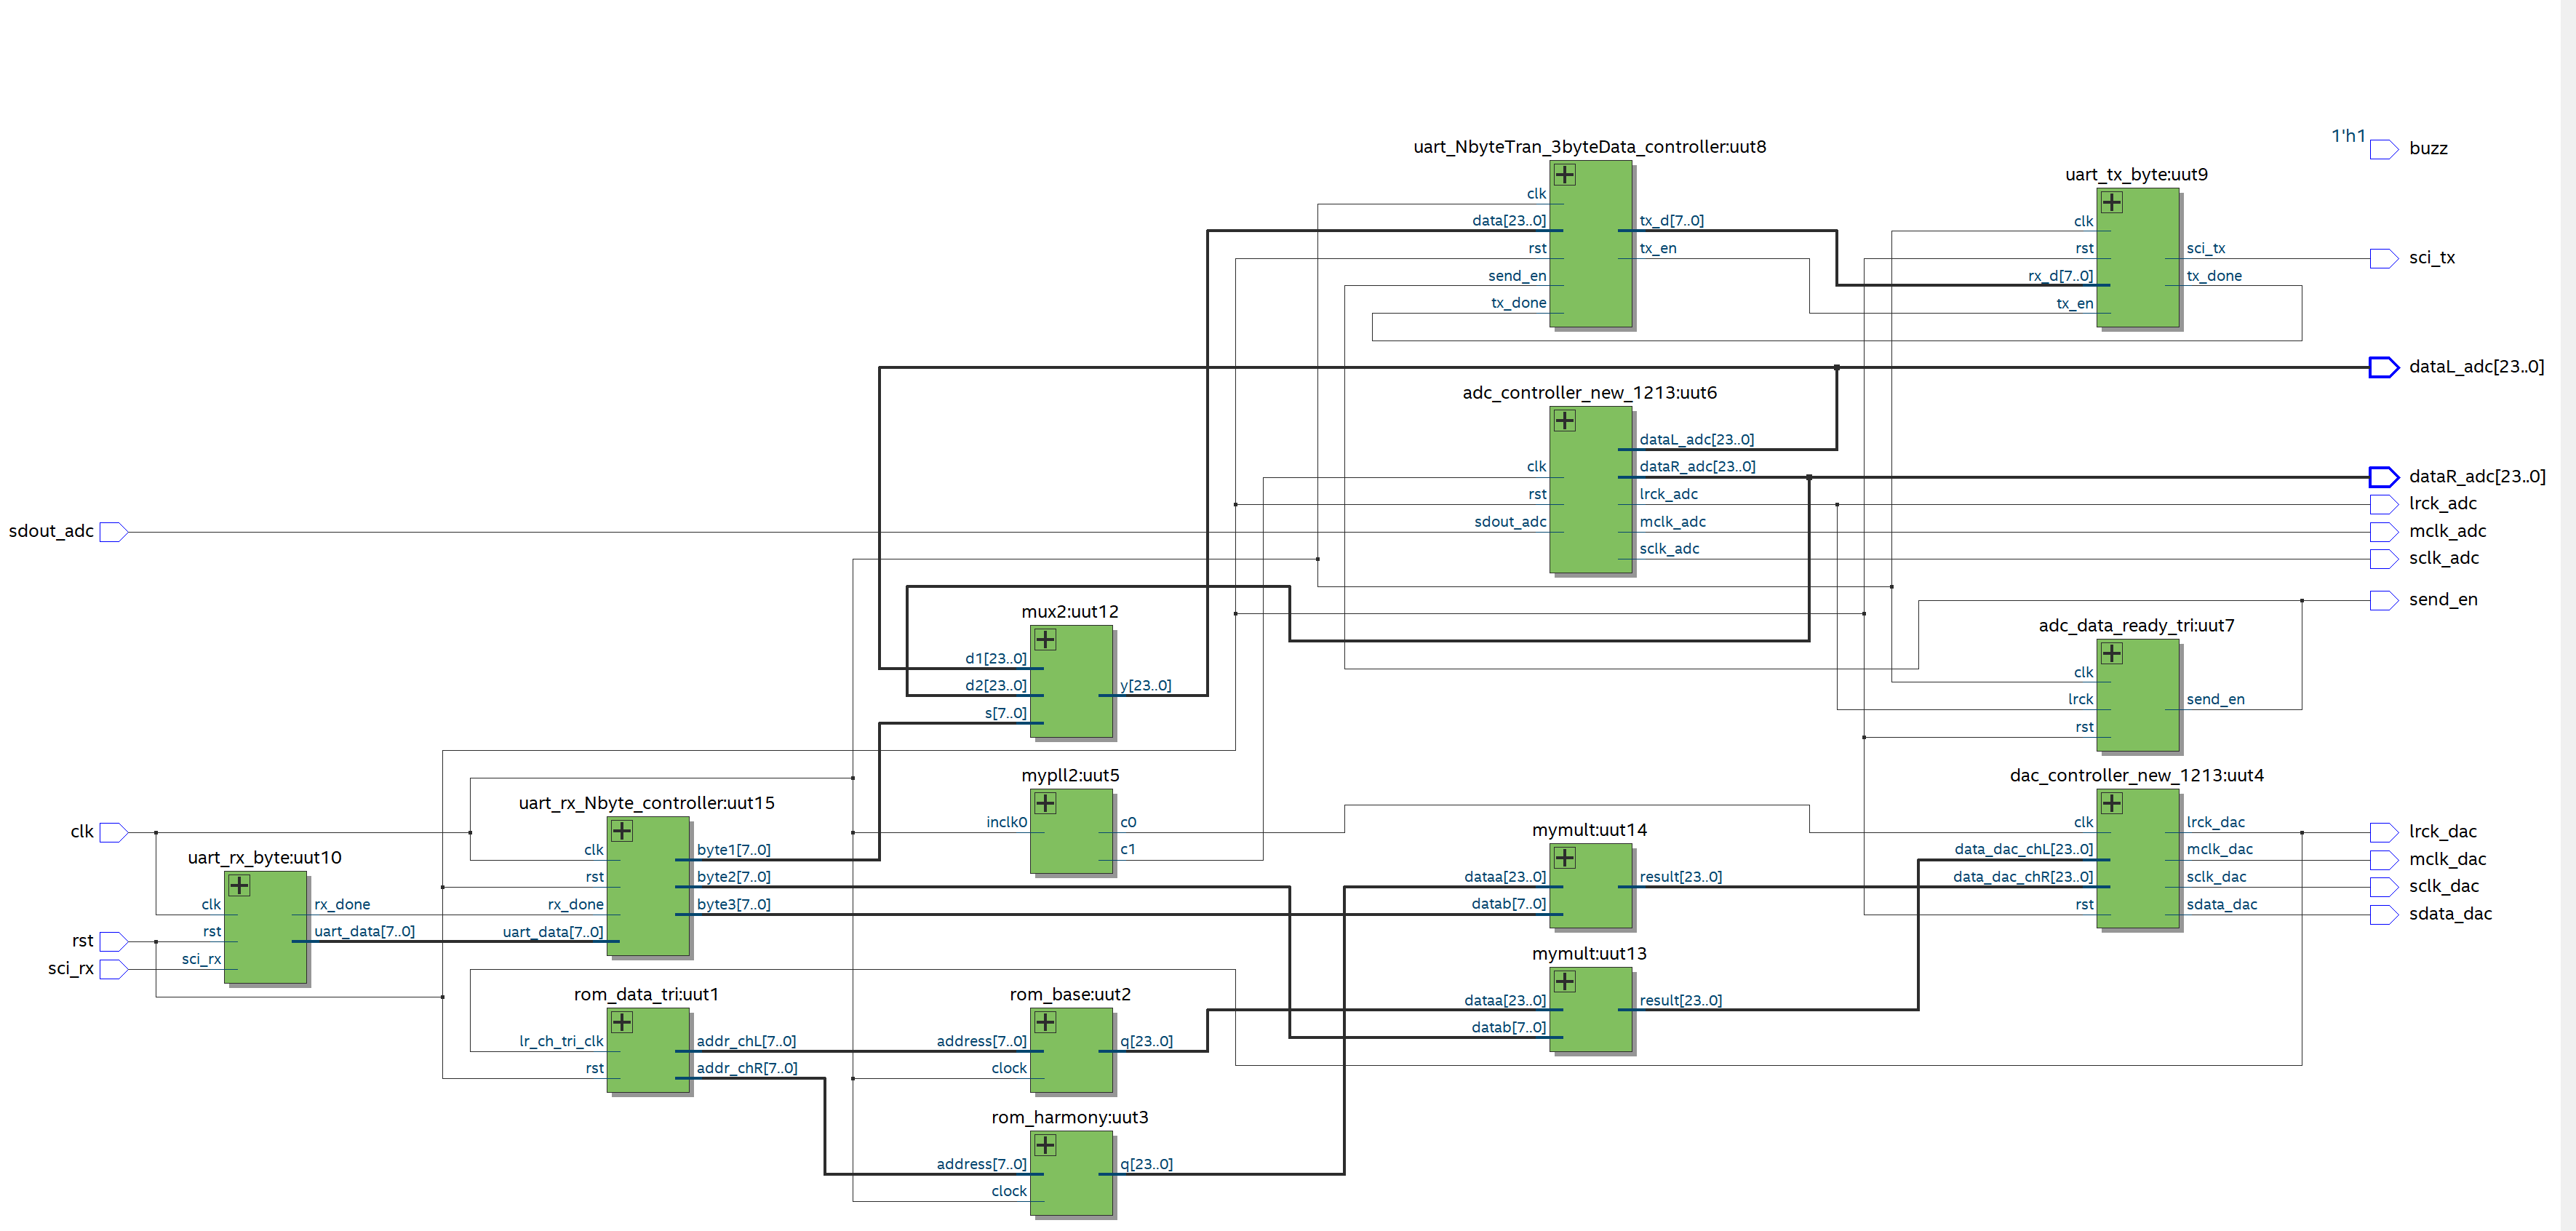
\includegraphics[width=\textwidth]{rtl3.png}
    \caption{task2顶层模块RTL电路图}
    \label{fig:rtl3}
\end{figure}

\subsection{仿真结果}
按照ppt中的要求,搭建simulink仿真模型,如图\ref{fig:simulink}所示。
\begin{figure}[!ht]
    \centering
    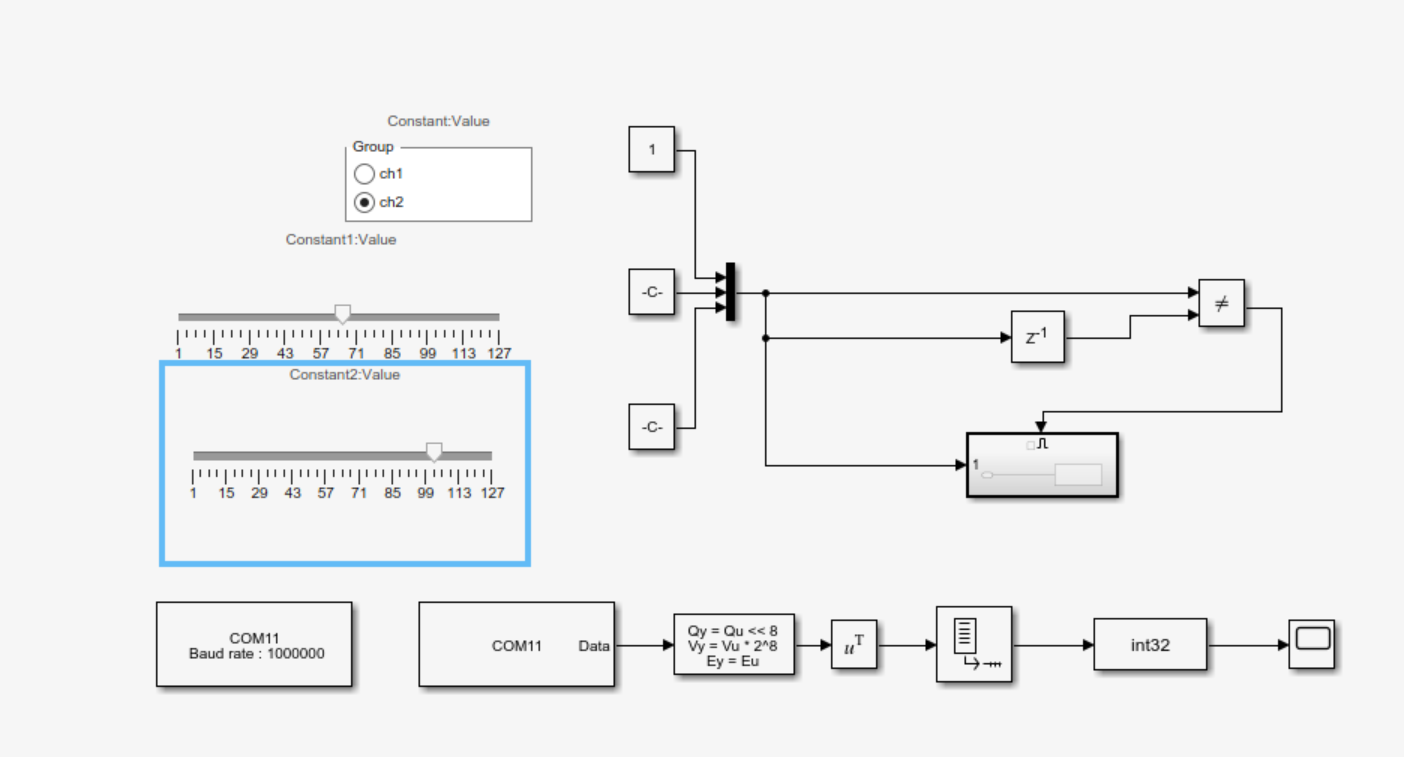
\includegraphics[width=\textwidth]{simulink.png}
    \caption{simulink仿真模型}
    \label{fig:simulink}
\end{figure}

仿真结果如图\ref{fig:simulink_result}所示。

%一个有四个子图的图组,四个子图成正方排列

\begin{figure}[!ht]
    \centering
    \subfigure[波形图1]{
        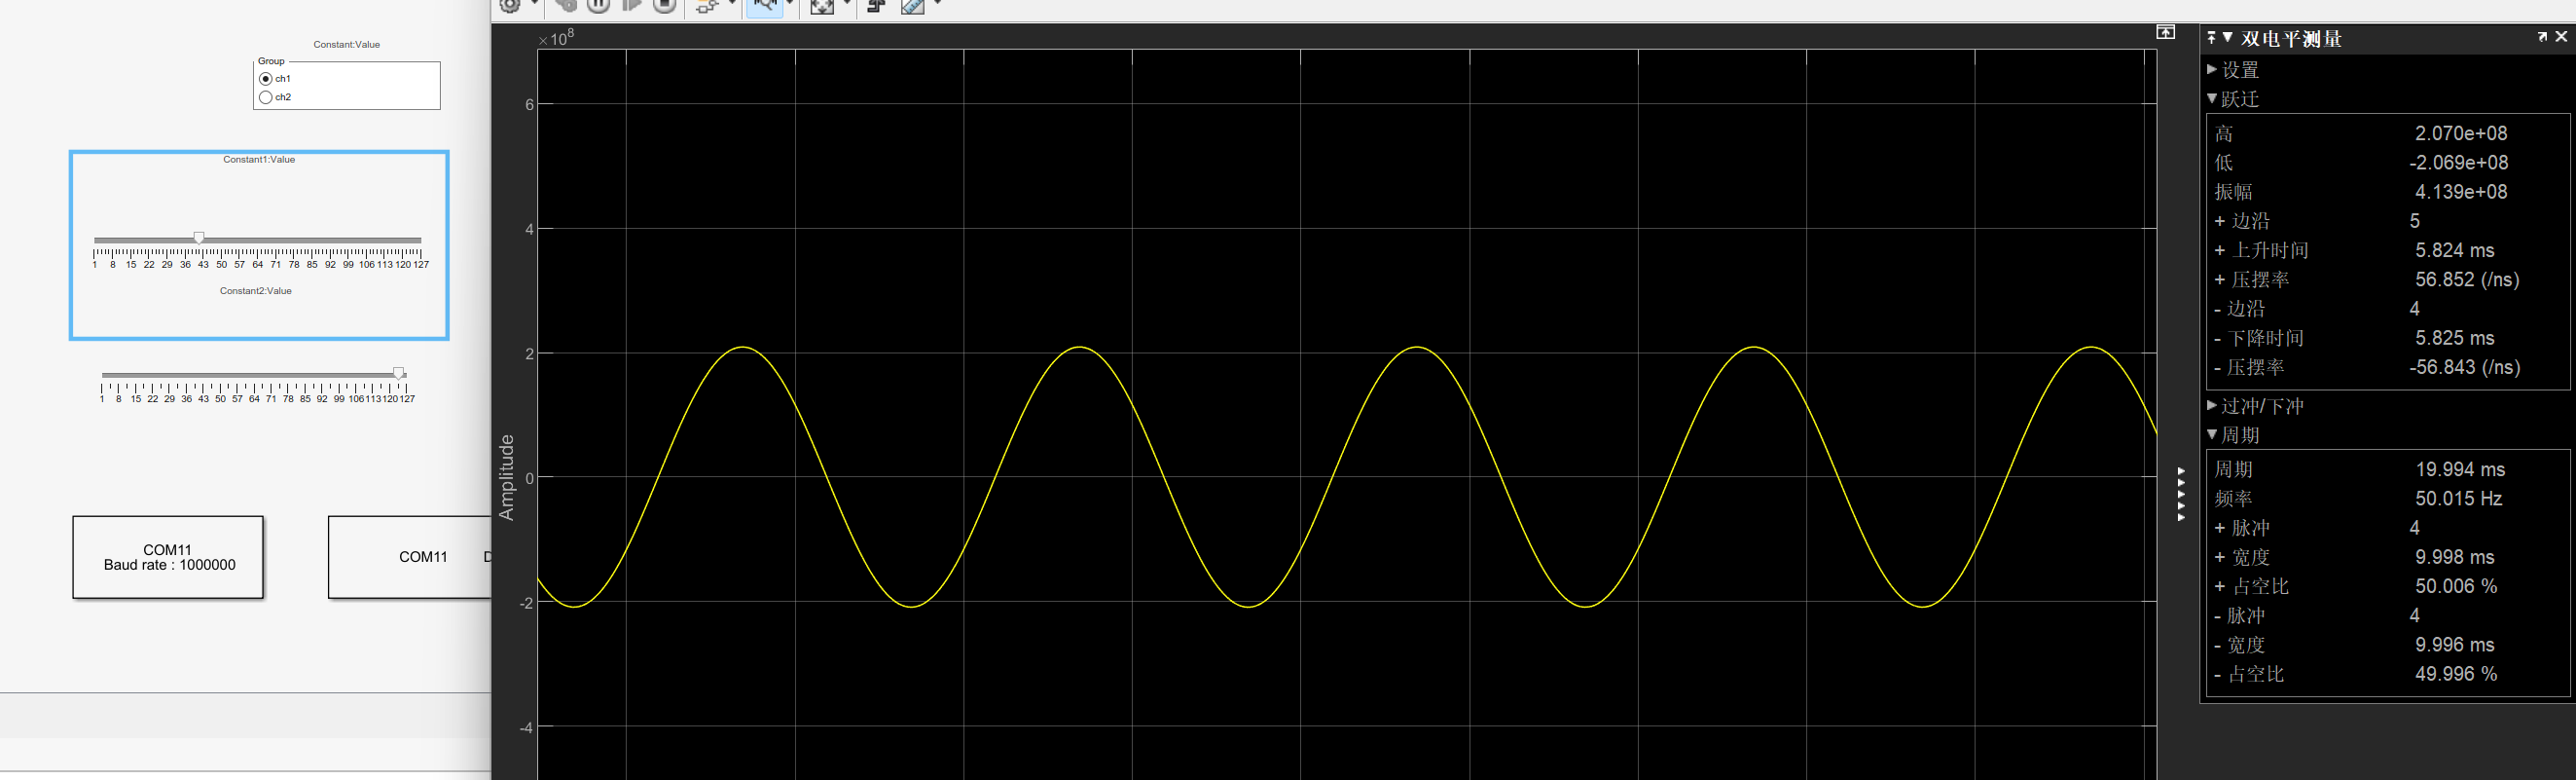
\includegraphics[width=0.45\textwidth]{simulink_result1.png}
    }
    \subfigure[波形图2]{
        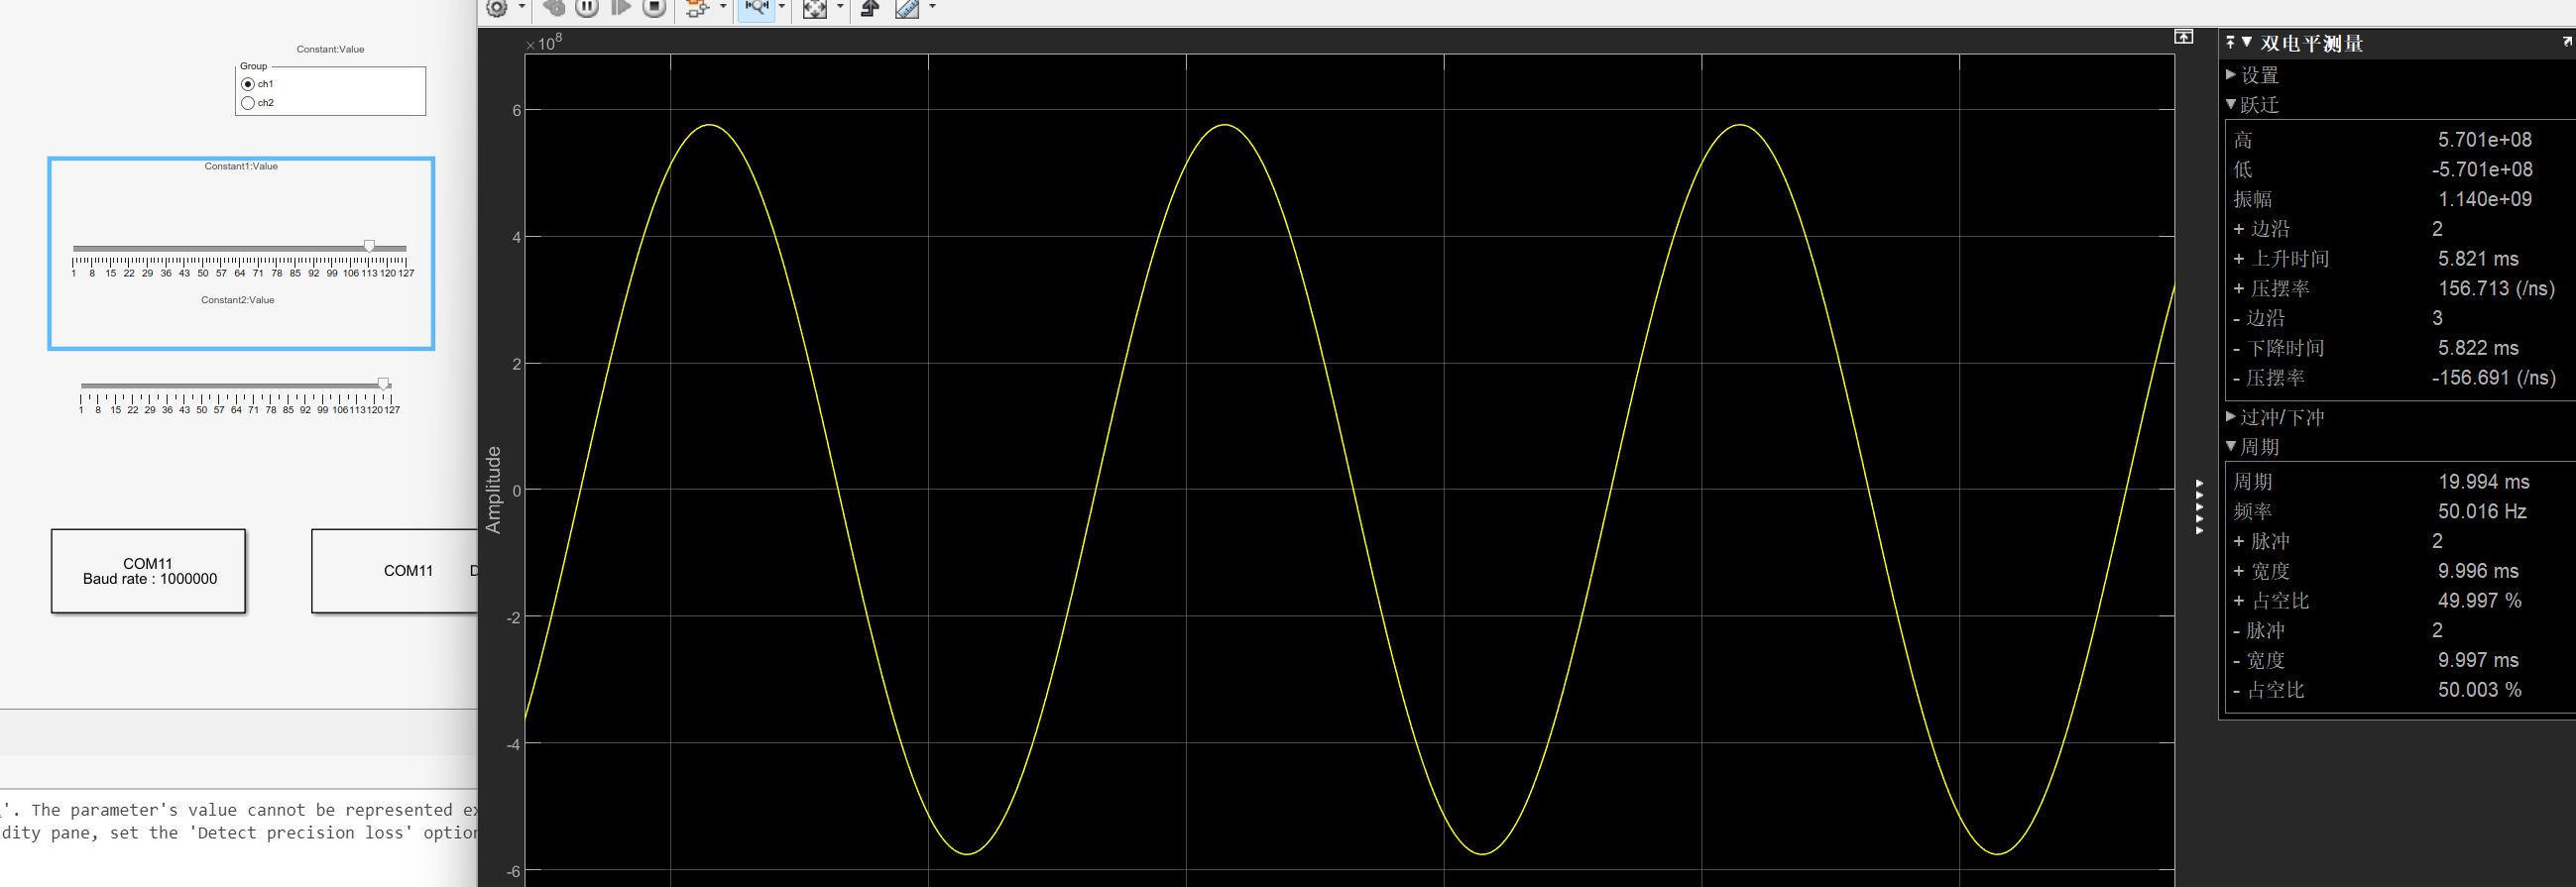
\includegraphics[width=0.45\textwidth]{simulink_result2.png}
    }
    \subfigure[波形图3]{
        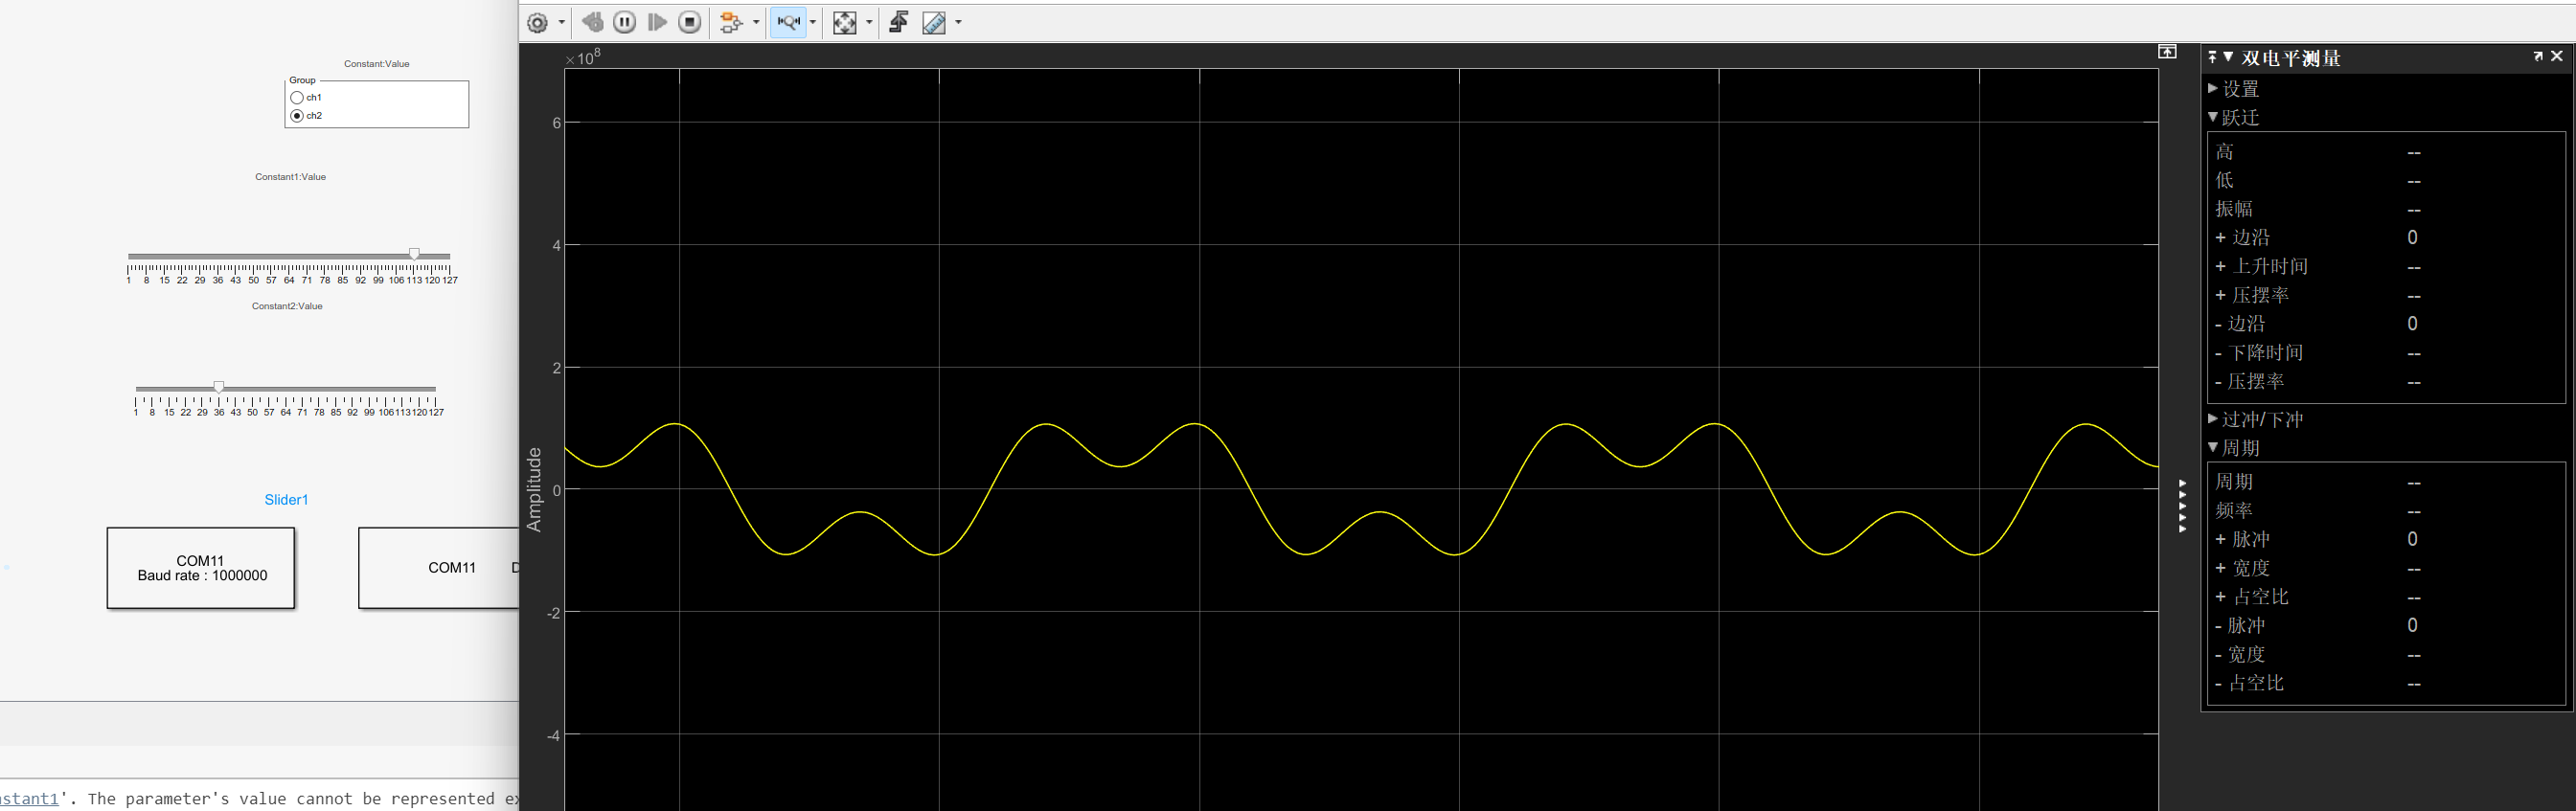
\includegraphics[width=0.45\textwidth]{simulink_result3.png}
    }
    \subfigure[波形图4]{
        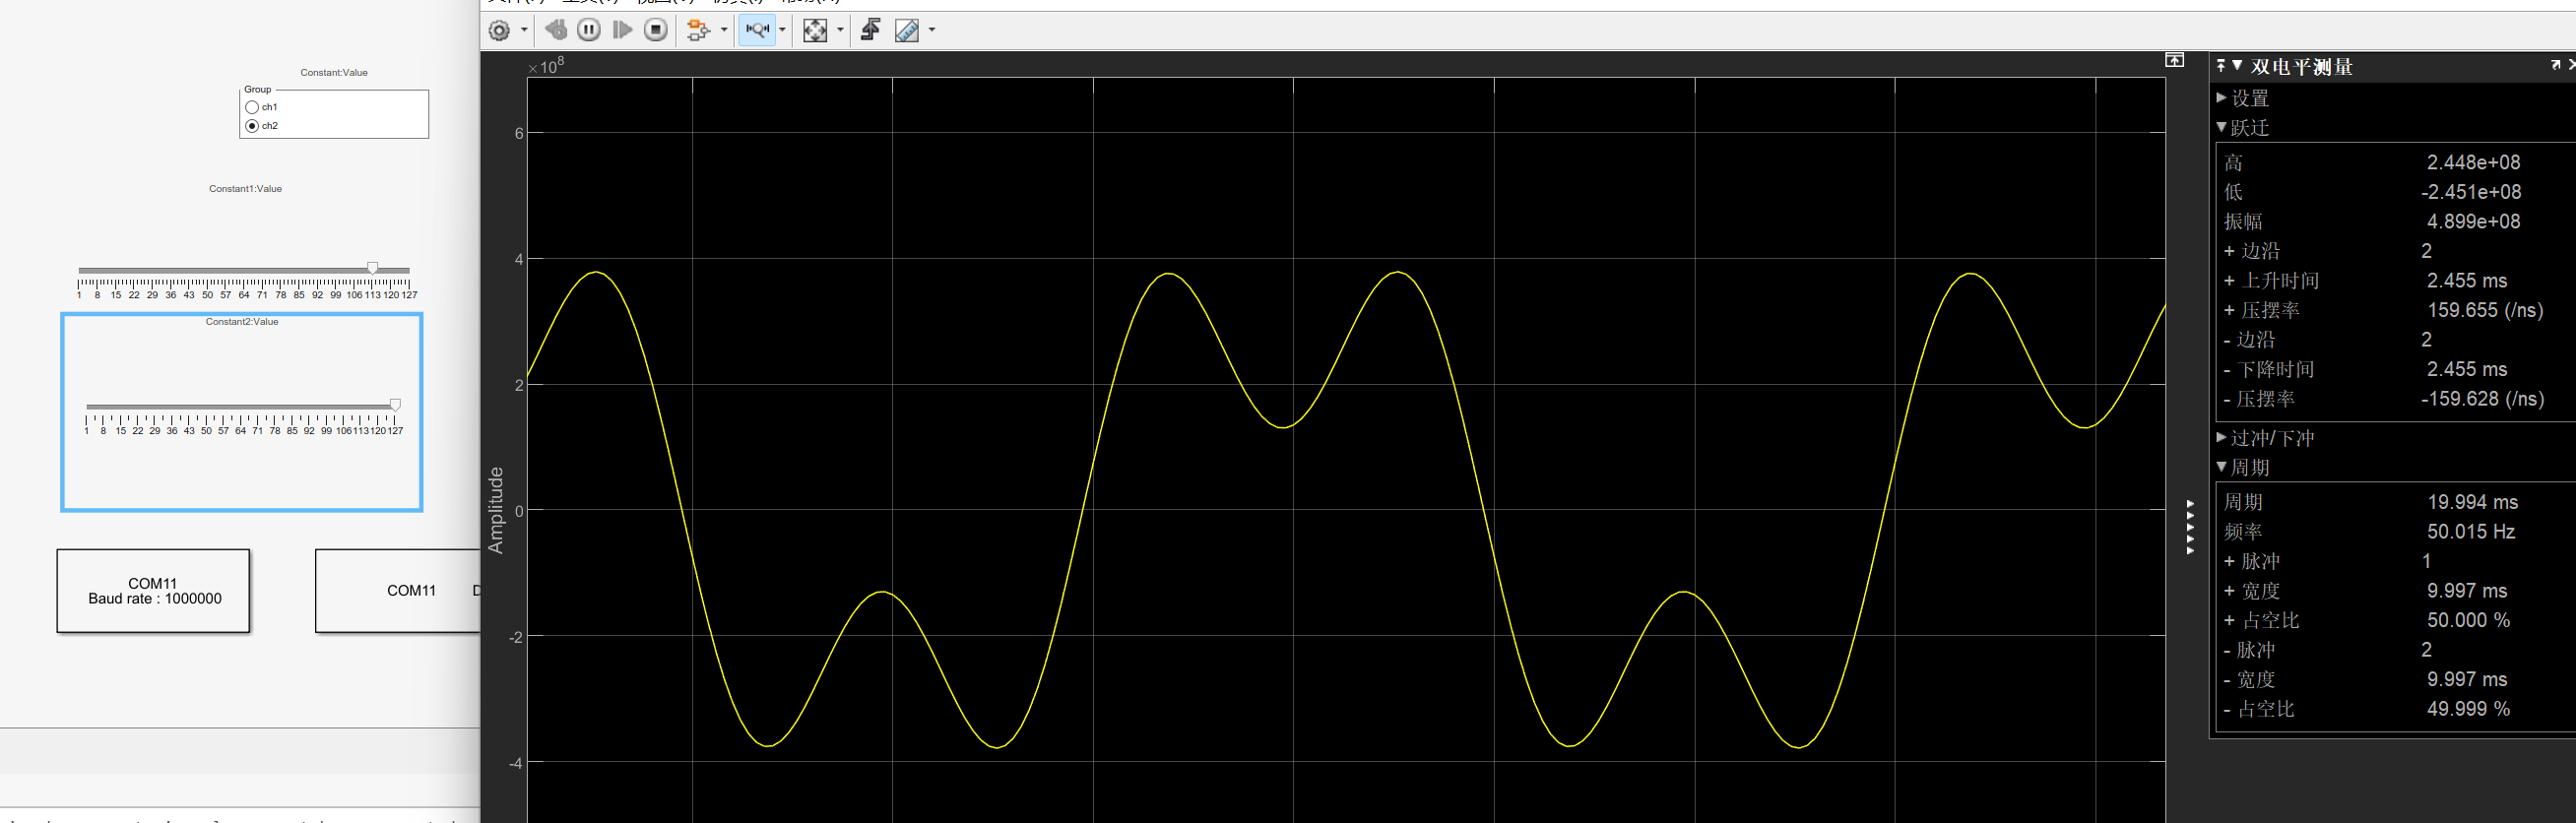
\includegraphics[width=0.45\textwidth]{simulink_result4.png}
    }
    \caption{simulink接收波形结果}
    \label{fig:simulink_result}
\end{figure}

可以看出通过选择channel,可以选择输出的信号。同时调节滑块可以调节输出波形的赋值。



\end{document}